\documentclass{praktikum}
\usepackage{graphicx}
\usepackage{caption}
\usepackage{subcaption}
\graphicspath{ {./} }
\usepackage{pgfplotstable}
%====== Vyplňte údaje ======
%% dobrá rada na začátek - pokud nevíš, co měníš, zálohuj to, co funguje ;)

\jmeno{Matyáš Peroutík}
\kod{256371}
\rocnik{1}
\obor{AMT}
\skupina{}
\labskup{B}
\spolupracoval{Štěpán Pavlica}


\ucitel{}
\merenodne{03.\,04.\,2024}
\odevzdanodne{10.\,04.\,2024}

\priprava{}
\opravy{}
\nazev{Měření magnetického pole přímých vodičů}
\cislo{52} %měřené úlohy

\usepackage{fancyhdr}
\usepackage{lastpage}
\pagestyle{fancy}
\fancyhf{}
\renewcommand{\headrulewidth}{0pt}
 
\rfoot{Strana \thepage \hspace{1pt} z \pageref{LastPage}}

\begin{document}

%====== Vygenerování tabulky ======
\maketitle
\vspace{0.5 cm}

%====== Text protokolu zde ======

\section{Úkol měření}
\begin{enumerate}
\item U přímého vodiče proměřte závislost velikosti elektromagnetické indukce na velikosti vodičem procházejícího elektrického proudu.
\item Při konstantní velikosti proudu procházejícího vodičem měřte změnu velikosti elektromagnetické indukce v závislosti na změně vzdálenosti
od vodiče.
\item Měřte velikost magnetické indukce v prostoru mezi dvěma paralelními
vodiči, kterými protéká elektrický proud stejným směrem a kterými poté protéká elektrický proud směry navzájem opačnými.

\end{enumerate}
\section{Teoretický rozbor}
\paragraph{}
Magnetické pole vznikne pouze tam, kde se pohybují elektrické náboje. Veličina popisující magnetické pole se nazývá indukce magnetického pole (nebo také magnetická indukce) a značí se $\vec{B}$. Magnetické pole lze jednoduše znázornit magnetickými indukčními čarami, což jsou orientované uzavřené, neprotínající se křivky, jejichž tečna má směr vektoru magnetické indukce. 

\indent Na částici s velikostí náboje q a rychlostí $\vec{v}$ v magnetickém poli o intenzitě $\vec{B}$ působí Lorenzova síla, která je dána následujícím vztahem:
\begin{equation}
\label{eqn:lorenz_force}
\vec{F_m}=q\vec{v}\times\vec{B}
\end{equation} 

Pokud se zde zároveň nachází vnější elektrické pole o intenzitě $\vec{E}$ je nutno přičíst sílu elektrickou, která je dána následujícím vztahem

\begin{equation}
\label{eqn:electric_force}
\vec{F_e} = q\vec{E}
\end{equation}

Po součtu těchto dvou sil dostaneme vzorec pro celkouvou sílu působící na částici.

\begin{equation}
\label{lorenz_electric_sumforce}
\vec{F} = q(\vec{E}+\vec{v}\times\vec{B})
\end{equation}

\indent Pro výpořet síly působící na vodič, který se nachází v magnetickém poli $\vec{B}$ vypočteme integrací z Apmerova zákona v diferenciálním tvaru.
\begin{equation}
\label{eqn:amper_dif_eqn}
d\vec{F} = Id\vec{l}\times\vec{B}
\end{equation}
Pokud se jedná o pole homogenní, lze vztah následovně zjednodušit:
\begin{equation}
\label{eqn:editted_amper_dif_eqn}
F = I\cdot l \cdot B \cdot sin\alpha
\end{equation}

Pokud vodičem protéká proud, můžeme magnetické pole v okolí tohoto vodiče popsat Biotovým-Savartovým zákonem. Dle něj je magnetická indukce $d\vec{B}$ vytvořená proudovým elementem $Id\vec{l}$ ve vzdálenosti r od tohoto elementu dána vztahem:

\begin{equation}
\label{eqn:biot_savrat_eqn}
d\vec{B} = \frac{\mu _0}{4\pi} \cdot \frac{I\cdot d\vec{l}\times \vec{r}}{r^3}
\end{equation}

\indent Pro velikost magnetické indukce ve vzdálenosti \textit{a} od přímého dlouhého vodiče lze ze vztahu (\ref{eqn:biot_savrat_eqn}) pomocí integrace odvodit následující vztah:

\begin{equation}
\label{eqn:long_wire_biot_savrat}
B = \frac{\mu _0 I}{2\pi a}
\end{equation}

Při použití tohoto vztahu je směr magnetického pole určen pomocí pravidla pravé ruky.

\section{Zpracování naměřených hodnot}

\subsection{Přímý vodič}

        \begin{figure}[H]
                         \begin{minipage}[b]{.45\textwidth}
    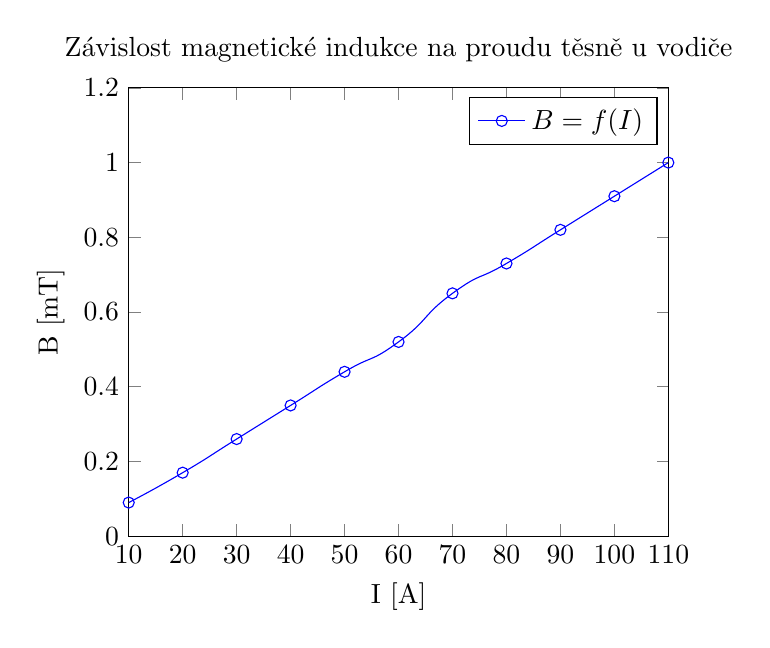
\begin{tikzpicture}[]

\begin{axis}[
    title={Závislost magnetické indukce na proudu těsně u vodiče},
    xlabel={I [A]},
    ylabel={B [mT]},
    xmin=10, xmax=110,
    ymin=0, ymax=1.2,
    xtick={10,20,30,40,50,60,70,80,90,100,110},
]

\addplot[
    color=blue,
    mark=o,
    smooth, tension=01,
    ]
    coordinates {
    (10, 0.09)
    (20, 0.17)
    (30, 0.26)
    (40, 0.35)
    (50, 0.44)
    (60, 0.52)
    (70, 0.65)
    (80, 0.73)
    (90, 0.82)
    (100,0.91)
    (110, 1)
    };
    \addlegendentry{$B=f(I)$}

    

    
\end{axis}
\end{tikzpicture}


  \end{minipage}\hfill
  \begin{minipage}[b]{.35\textwidth}
% Please add the following required packages to your document preamble:
% \usepackage{graphicx}
\begin{table}[H]
\centering
\resizebox{.45\textwidth}{!}{%
\begin{tabular}{|c|c|}
\hline
\textbf{I}       & \textbf{B}        \\ \hline
\textit{{[}A{]}} & \textit{{[}mT{]}} \\ \hline
10               & 0.09              \\ \hline
20               & 0.17              \\ \hline
30               & 0.26              \\ \hline
40               & 0.35              \\ \hline
50               & 0.44              \\ \hline
60               & 0.52              \\ \hline
70               & 0.65              \\ \hline
80               & 0.73              \\ \hline
90               & 0.82              \\ \hline
100              & 0.91              \\ \hline
110              & 1                 \\ \hline
\end{tabular}%
}
\caption{Tabulka naměřených hodnot B = f(I)}
\label{tab:namerene_bfi}
\end{table}
  \end{minipage}
                        \end{figure}\newpage

\indent Výpočtem z průměrných hodnot zde můžeme určit teoretickou vzdálenost sondy od vodiče.

\begin{equation}
\label{eqn:calc_singlewire_distance}
a=\frac{\mu _0\overline{I}}{2\pi\overline{B}}=\frac{\mu _0 \cdot 60}{2 \pi \cdot 0.54 \cdot 10^{-3}} \doteq 0.02222m \doteq 22.22mm
\end{equation}

\indent Počítat z průměrných hodnot můžeme, protože magnetická indukce je přímo ůměrná proudu. Pokud budeme tuto hodnotu vzdálenosti uvažovat jako výchozí, můžeme spočítat teoretické hodnoty pro tento průběh v závislosti na proudu. Pro hodnotu např. \textit{I=100A} bude výpočet podle vztahu (\ref{eqn:long_wire_biot_savrat}) vypadat následovně:
\[ B = \frac{\mu _0 \cdot 100}{2\pi \cdot 0.02222} = 0.9mT \]

\indent Zde lze vidět, že odchylka od naměřené je minimální. Pokud tedy s touto hodnotou dopočteme zbytek tabulky a necháme ji vygrafovat, dostaneme následující tabulku a průběh.

        \begin{figure}[H]
                         \begin{minipage}[b]{.45\textwidth}
    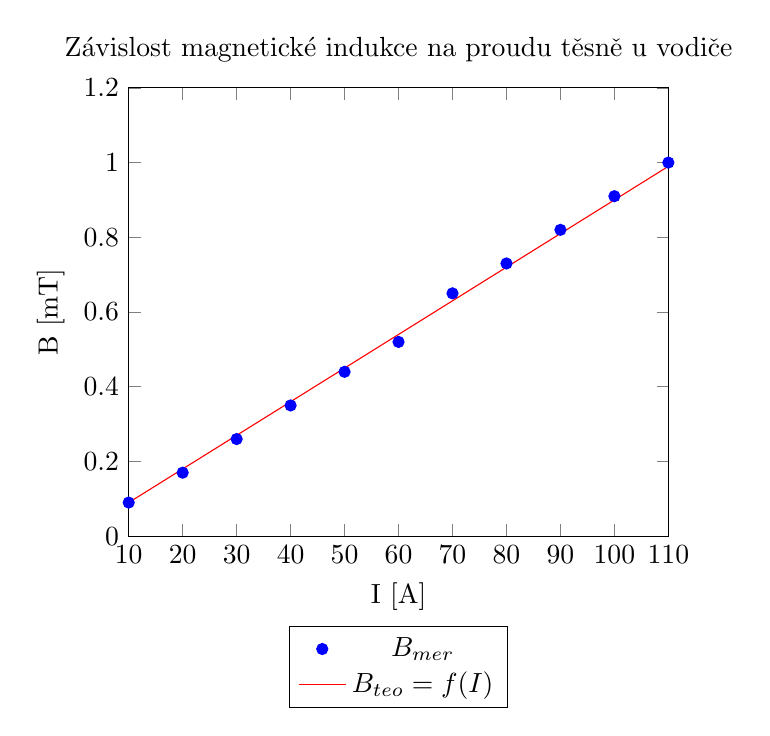
\begin{tikzpicture}[]
\pgfplotsset{
every axis legend/.append style={ at={(0.5,-0.2)}, anchor=north,legend columns = 1}}
\begin{axis}[
    title={Závislost magnetické indukce na proudu těsně u vodiče},
    xlabel={I [A]},
    ylabel={B [mT]},
    xmin=10, xmax=110,
    ymin=0, ymax=1.2,
    xtick={10,20,30,40,50,60,70,80,90,100,110},
]
\addplot[
    color=blue,
   	only marks
    ]
    coordinates {
    (10, 0.09)
    (20, 0.17)
    (30, 0.26)
    (40, 0.35)
    (50, 0.44)
    (60, 0.52)
    (70, 0.65)
    (80, 0.73)
    (90, 0.82)
    (100,0.91)
    (110, 1)
    };
    \addlegendentry{$B_{mer}$}
\addplot[
    color=red,
   	no marks
    ]
    coordinates {
    (10, 0.09)
    (20, 0.18)
    (30, 0.27)
    (40, 0.36)
    (50, 0.45)
    (60, 0.54)
    (70, 0.63)
    (80, 0.72)
    (90, 0.81)
    (100,0.9)
    (110, 0.99)
    };
    \addlegendentry{$B_{teo} = f(I)$}
    

    
\end{axis}
\end{tikzpicture}


  \end{minipage}\hfill
  \begin{minipage}[b]{.35\textwidth}
% Please add the following required packages to your document preamble:
% \usepackage{graphicx}
\begin{table}[H]
\centering
\resizebox{.75\textwidth}{!}{%
\begin{tabular}{|c|c|c|}
\hline
\textbf{I}       & \textbf{B$_{mer}$} &\textbf{B$_{teo}$}       \\ \hline
\textit{{[}A{]}} & \textit{{[}mT{]}}& \textit{{[}mT{]}} \\ \hline
10               & 0.09     & 0.09         \\ \hline
20               & 0.17     & 0.18     \\ \hline
30               & 0.26     & 0.27         \\ \hline
40               & 0.35     & 0.36        \\ \hline
50               & 0.44     & 0.45         \\ \hline
60               & 0.52     & 0.54         \\ \hline
70               & 0.65     & 0.63         \\ \hline
80               & 0.73     & 0.72         \\ \hline
90               & 0.82     & 0.81         \\ \hline
100              & 0.91     & 0.9         \\ \hline
110              & 1        & 0.99         \\ \hline
\end{tabular}%
}
\caption{Tabulka naměřených hodnot B = f(I)}
\label{tab:namerene_bfi_teo}
\end{table}
  \end{minipage}
  \end{figure}



\subsection{Paralelní vodiče - nesouhlasný směr}


\begin{table}[H]
\centering
\resizebox{0.55\textwidth}{!}{%
\begin{tabular}{|c|c|c|c|c|c|c|c|}
\hline
\textbf{a}        & \textbf{B}        &           & \textbf{a}        & \textbf{B}        &           & \textbf{a}        & \textbf{B}        \\ \hline
\textit{{[}mm{]}} & \textit{{[}mT{]}} & \textit{} & \textit{{[}mm{]}} & \textit{{[}mT{]}} & \textit{} & \textit{{[}mm{]}} & \textit{{[}mT{]}} \\ \hline
-100 & 0.06 &  & -25 & 1.34 &  & 33  & 1.44 \\ \hline
-90  & 0.05 &  & -21 & 0.89 &  & 37  & 1.67 \\ \hline
-80  & 0.04 &  & -17 & 0.62 &  & 41  & 1.55 \\ \hline
-70  & 0.02 &  & -13 & 0.41 &  & 45  & 1.15 \\ \hline
-65  & 0.04 &  & -9  & 0.25 &  & 49  & 0.80 \\ \hline
-61  & 0.06 &  & -5  & 0.15 &  & 51  & 0.54 \\ \hline
-57  & 0.10 &  & -0  & 0.06 &  & 57  & 0.40 \\ \hline
-53  & 0.15 &  & 5   & 0.04 &  & 61  & 0.29 \\ \hline
-49  & 0.28 &  & 9   & 0.11 &  & 65  & 0.2  \\ \hline
-45  & 0.45 &  & 13  & 0.22 &  & 70  & 0.14 \\ \hline
-41  & 0.70 &  & 17  & 0.32 &  & 80  & 0.06 \\ \hline
-37  & 1.08 &  & 21  & 0.43 &  & 90  & 0.03 \\ \hline
-33  & 1.51 &  & 25  & 0.67 &  & 100 & 0.03 \\ \hline
-29  & 1.67 &  & 29  & 1.01 &  &     &      \\ \hline
\end{tabular}%
}
\caption{Tabulka naměřených hodnot B = f(a) při I=100A dvou paralelních nesouhlasných vodičů}
\label{tab:namerene_hodnoty_bfa_n}
\end{table}

\begin{figure}[H]
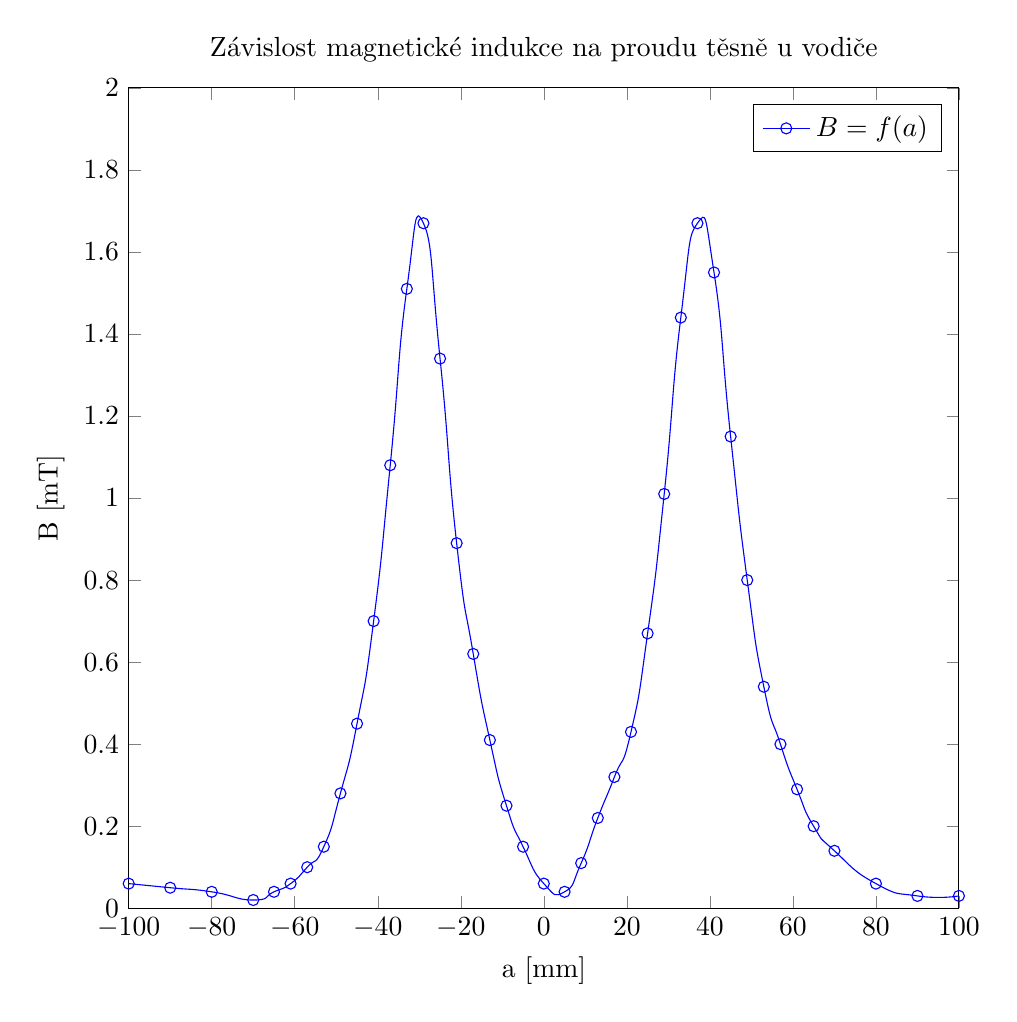
\begin{tikzpicture}[]

\begin{axis}[
    title={Závislost magnetické indukce na proudu těsně u vodiče},
    width=\textwidth,
    height= 12cm,
    xlabel={a [mm]},
    ylabel={B [mT]},
    xmin=-100, xmax=100,
    ymin=0, ymax=2,
    xtick={-100, -80, -60, -40, -20, 0, 20 ,40, 60, 80, 100},
]

\addplot[
    color=blue,
    mark=o,
    smooth, tension=01,
    ]
    coordinates {
    (-100,0.06)
    (-90, 0.05)
    (-80, 0.04)
    (-70, 0.02)
    (-65, 0.04)
    (-61, 0.06)
    (-57, 0.10)
    (-53, 0.15)
    (-49, 0.28)
    (-45, 0.45)
    (-41, 0.70)
    (-37, 1.08)
    (-33, 1.51)
    (-29, 1.67)
    (-25, 1.34)
    (-21, 0.89)
    (-17, 0.62)
    (-13, 0.41)
    (-9,  0.25)
    (-5,  0.15)
    (0,  0.06)
    (5,  0.04)
    (9,  0.11)
    (13, 0.22)
    (17, 0.32)
    (21, 0.43)
    (25, 0.67)
    (29, 1.01)
    (33, 1.44)
    (37, 1.67)
    (41, 1.55)
    (45, 1.15)
    (49, 0.80)
    (53, 0.54)
    (57, 0.40)
    (61, 0.29)
    (65, 0.20)
    (70, 0.14)
    (80, 0.06)
    (90, 0.03)
    (100,0.03)
    };
    \addlegendentry{$B=f(a)$}

\end{axis}
\end{tikzpicture}
\end{figure}

\subsubsection{Odvození vztahu pro teoretickou hodnotu magnetické indukce nesouhlasného směru proudů}
\paragraph{}
Vzdálenost \textit{a} (viz tab.) je vzdálenost po ose pohybu sondy, nikoliv vzdálenost od vodiče. Proto musíme uvažovat skutečnou vzdálenost od středu vodiče jako

\begin{equation}
\label{eqn:calc_real_distance}
a_{r} = \sqrt{a^2 + a_v^2}
\end{equation} kde $a_r$ je vzdálenost po ose posuvu sondy od maxima daného vodiče, a $a_v$ je vzdálenost osy hallovy sondy průsečnice středů vodičů\\

Pro získání teoretických hodnot průběhu budeme uvažovat, že osa pohybu sondy byla rovnoběžná s průsečnicí středů vodičů. Tuto vzdálenost spočteme z průměru maximálních hodnot při proudu 100A odvozením ze vztahu (\ref{eqn:long_wire_biot_savrat}). Jelikož působí oba vodiče zároveň, musíme při výpočtu vzdálenosti také uvažovat působení síly druhého vodiče.\\ Jelikož hallova sonda, kterou bylo prováděno měření, měřila pravděpodobně pouze v jedné ose, a velikost magnetické indukce je vektorová veličina, vynásobíme vztah (\ref{eqn:long_wire_biot_savrat}) navíc kosinem úhlu, který svírá s hranou měřidla, kterou jsem určil, že je kolmá na osu pohybu. Tento kosinus bude poté poměr vzdálenosti $a_v$ a $a_r$. Pro polohu -29mm (resp. přímo u 1. vodiče), při které je B=1.67mT bude tedy platit následující vztah:

\[ 1.67 \cdot 10^{-3} = \frac{\mu _0 \cdot 100\cdot \frac{a_v}{\sqrt{a_v^2+(-0.029+0.029)^2}}}{2\pi \cdot \sqrt{a_v^2 + (-29-(-29))^2}} - \frac{\mu _0 \cdot 100\cdot \frac{a_v}{\sqrt{a_v^2+(-0.029-0.037)^2}}}{2\pi \cdot \sqrt{a_v^2 + ((-29-37)\cdot 10^{-3})^2}} \]

\[ 1.67 \cdot 10^{-3} = 2 \cdot 10^{-7} \cdot 100 \cdot \left(\frac{1}{a_v} - \frac{\frac{a_v}{\sqrt{a_v^2+0.066^2}}}{\sqrt{a_v^2 + (-0.066^2)}}\right) \]

Numerickým řešením pro $a_v$ dostaneme následující hodnotu vzdálenosti osy pohybu hallovy sondy:

\begin{equation}
\label{eqn:calc_opositewire_distance}
a_v=0.01238m=12.38mm
\end{equation}



Jelikož ve vodičích prochází proud opačnými směry, musíme je mezi sebou odečíst. Vzdálenost musíme uvádět vždy jako vzdálenost od určitého maxima příslušného vodiče. Tyto maxima budeme uvažovat jako -29mm a 37mm pro 1. a 2. vodič respektivě. Zjednodušením vztahu (\ref{eqn:long_wire_biot_savrat}) dostaneme následující vztah pro libovolnou teoretickou hodnotu indukce na sondě ve vzdálenosti na měřítku sondy při proudu 100A.

\begin{equation}
\label{eqn:calc_oppositewire_magnetic}
B_a = 2 \cdot 10^{-7} \cdot 100 \cdot \left(\frac{\frac{a_v}{\sqrt{a_v^2+(a+0.029)^2}}}{\sqrt{0.01238^2 + (a+0.029)^2}} - \frac{\frac{a_v}{\sqrt{a_v^2+(a-0.037)^2}}}{\sqrt{0.01238^2 + (a-0.037)^2}}\right)
\end{equation}

Pomocí tohoto vztahu jsme schopni dopočítat teoretické hodnoty magnetické indukce. Následně je ukázáno jak se vypočatla hodnota pro a=0mm.

\[ B_0 = 2 \cdot 10^{-7} \cdot 100 \cdot \left(\frac{0.39}{\sqrt{0.01238^2 + (0+0.029)^2}} - \frac{0.31}{\sqrt{0.01238^2 + (0-0.037)^2}}\right) \]

\[B_0  = 0.41 mT\]

% Please add the following required packages to your document preamble:
% \usepackage{graphicx}
\begin{table}[H]
\centering
\resizebox{0.8\columnwidth}{!}{%
\begin{tabular}{|c|c|l|c|c|c|l|c|c|c|l|}
\hline
\textbf{a} &
  \textbf{B}$_{mer}$ &
  \multicolumn{1}{c|}{\textbf{B}$_{teo}$} &
   &
  \textbf{a} &
  \textbf{B}$_{mer}$ &
  \multicolumn{1}{c|}{\textbf{B}$_{teo}$} &
   &
  \textbf{a} &
  \textbf{B}$_{mer}$ &
  \multicolumn{1}{c|}{\textbf{B}$_{teo}$} \\ \hline
\textit{{[}mm{]}} &
  \textit{{[}mT{]}} &
  \multicolumn{1}{c|}{\textit{{[}mT{]}}} &
  \textit{} &
  \textit{{[}mm{]}} &
  \textit{{[}mT{]}} &
  \multicolumn{1}{c|}{\textit{{[}mT{]}}} &
  \textit{} &
  \textit{{[}mm{]}} &
  \textit{{[}mT{]}} &
  \multicolumn{1}{c|}{\textit{{[}mT{]}}} \\ \hline
-100 & 0.06 & 0.06 & \textbf{} & -25 & 1.34 & 1.52 & \textbf{} & 33  & 1.44 & 1.52 \\ \hline
-90  & 0.05 & 0.08 &           & -21 & 0.89 & 1.21 &           & 37  & 1.67 & 1.67 \\ \hline
-80  & 0.04 & 0.11 &           & -17 & 0.62 & 0.91 &           & 41  & 1.55 & 1.51 \\ \hline
-70  & 0.02 & 0.16 &           & -13 & 0.41 & 0.70 &           & 45  & 1.15 & 1.18 \\ \hline
-65  & 0.04 & 0.19 &           & -9  & 0.25 & 0.56 &           & 49  & 0.80 & 0.87 \\ \hline
-61  & 0.06 & 0.24 &           & -5  & 0.15 & 0.47 &           & 51  & 0.54 & 0.64 \\ \hline
-57  & 0.10 & 0.29 &           & 0  & 0.06 & 0.41 &           & 57  & 0.40 & 0.48 \\ \hline
-53  & 0.15 & 0.37 &           & 5   & 0.04 & 0.40 &           & 61  & 0.29 & 0.37 \\ \hline
-49  & 0.28 & 0.48 &           & 9   & 0.11 & 0.42 &           & 65  & 0.2  & 0.29 \\ \hline
-45  & 0.45 & 0.64 &           & 13  & 0.22 & 0.47 &           & 70  & 0.14 & 0.22 \\ \hline
-41  & 0.70 & 0.87 &           & 17  & 0.32 & 0.56 &           & 80  & 0.06 & 0.14 \\ \hline
-37  & 1.08 & 1.18 &           & 21  & 0.43 & 0.70 &           & 90  & 0.03 & 0.10 \\ \hline
-33  & 1.51 & 1.51 &           & 25  & 0.67 & 0.91 &           & 100 & 0.03 & 0.07 \\ \hline
-29  & 1.67 & 1.67 &           & 29  & 1.01 & 1.21 &           &     &      &      \\ \hline
\end{tabular}%
}
\caption{Tabulka naměřených a teoretických hodnot B = f(a) při I=100A}
\label{tab:namer_teo_bfa_opp}
\end{table}


\begin{figure}[H]
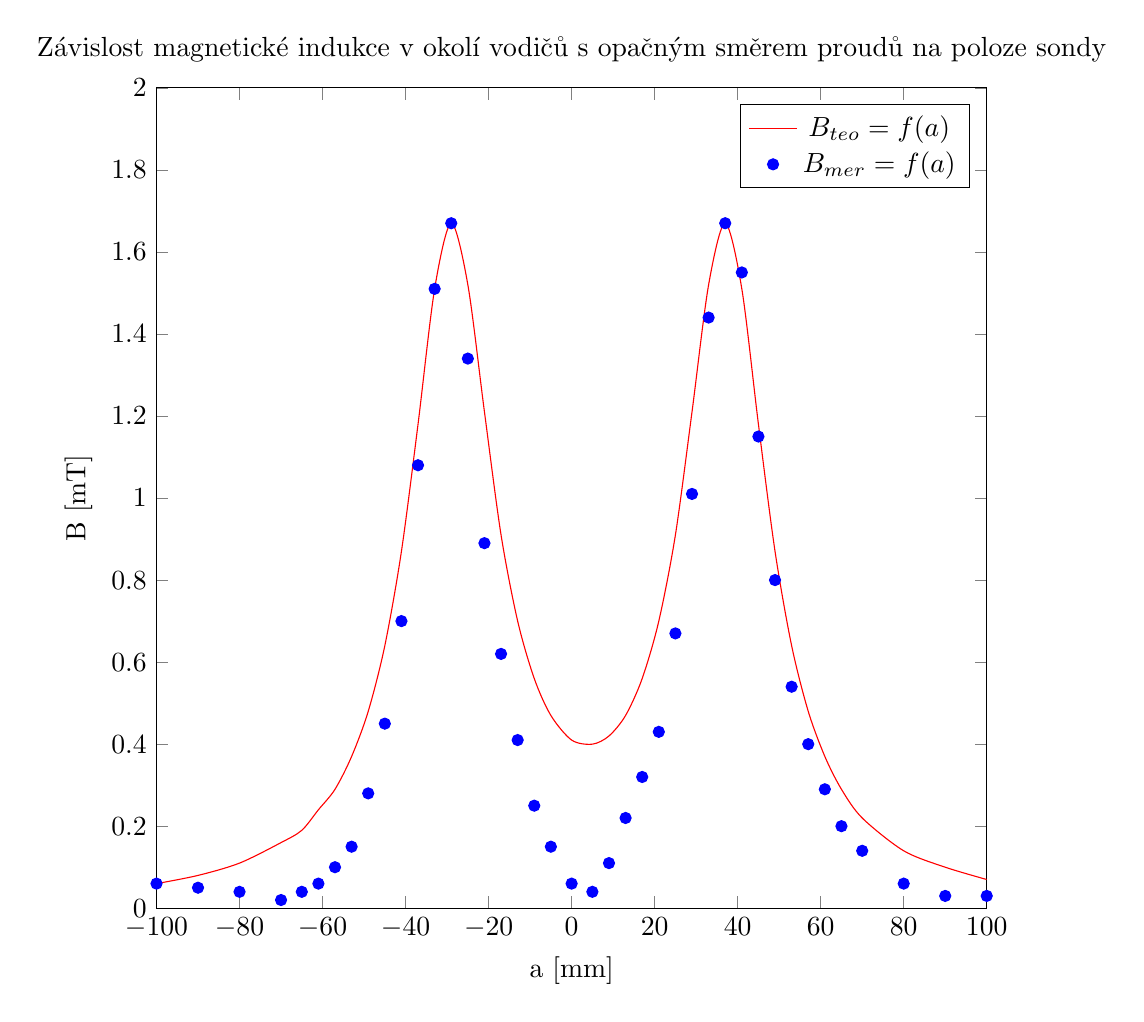
\begin{tikzpicture}[]

\begin{axis}[
    title={Závislost magnetické indukce v okolí vodičů s opačným směrem proudů na poloze sondy},
    width=\textwidth,
    height= 12cm,
    xlabel={a [mm]},
    ylabel={B [mT]},
    xmin=-100, xmax=100,
    ymin=0, ymax=2,
    xtick={-100, -80, -60, -40, -20, 0, 20 ,40, 60, 80, 100},
]
\addplot[
    color=red,
    smooth
    ]
    coordinates {
    (-100,0.06)
    (-90, 0.08)
    (-80, 0.11)
    (-70, 0.16)
    (-65, 0.19)
    (-61, 0.24)
    (-57, 0.29)
    (-53, 0.37)
    (-49, 0.48)
    (-45, 0.64)
    (-41, 0.87)
    (-37, 1.18)
    (-33, 1.51)
    (-29, 1.67)
    (-25, 1.52)
    (-21, 1.21)
    (-17, 0.91)
    (-13, 0.70)
    (-9,  0.56)
    (-5,  0.47)
    (0,  0.41)
    (5,  0.40)
    (9,  0.42)
    (13, 0.47)
    (17, 0.56)
    (21, 0.70)
    (25, 0.91)
    (29, 1.21)
    (33, 1.52)
    (37, 1.67)
    (41, 1.51)
    (45, 1.18)
    (49, 0.87)
    (53, 0.64)
    (57, 0.48)
    (61, 0.37)
    (65, 0.29)
    (70, 0.22)
    (80, 0.14)
    (90, 0.10)
    (100,0.07)
    };    
    \addlegendentry{$B_{teo}=f(a)$}
\addplot[
    color=blue,
    only marks
    ]
    coordinates {
    (-100,0.06)
    (-90, 0.05)
    (-80, 0.04)
    (-70, 0.02)
    (-65, 0.04)
    (-61, 0.06)
    (-57, 0.10)
    (-53, 0.15)
    (-49, 0.28)
    (-45, 0.45)
    (-41, 0.70)
    (-37, 1.08)
    (-33, 1.51)
    (-29, 1.67)
    (-25, 1.34)
    (-21, 0.89)
    (-17, 0.62)
    (-13, 0.41)
    (-9,  0.25)
    (-5,  0.15)
    (0,  0.06)
    (5,  0.04)
    (9,  0.11)
    (13, 0.22)
    (17, 0.32)
    (21, 0.43)
    (25, 0.67)
    (29, 1.01)
    (33, 1.44)
    (37, 1.67)
    (41, 1.55)
    (45, 1.15)
    (49, 0.80)
    (53, 0.54)
    (57, 0.40)
    (61, 0.29)
    (65, 0.20)
    (70, 0.14)
    (80, 0.06)
    (90, 0.03)
    (100,0.03)
    };
    \addlegendentry{$B_{mer}=f(a)$}
    
    
\end{axis}
\end{tikzpicture}
\end{figure}

\subsection{Paralelní vodiče - souhlasný směr}
% Please add the following required packages to your document preamble:
% \usepackage{graphicx}
\begin{table}[H]
\centering
\resizebox{0.55\columnwidth}{!}{%
\begin{tabular}{|c|c|c|c|c|c|c|c|}
\hline
\textbf{a}        & \textbf{B}        &           & \textbf{a}        & \textbf{B}        &           & \textbf{a}        & \textbf{B}        \\ \hline
\textit{{[}mm{]}} & \textit{{[}mT{]}} & \textit{} & \textit{{[}mm{]}} & \textit{{[}mT{]}} & \textit{} & \textit{{[}mm{]}} & \textit{{[}mT{]}} \\ \hline
-100 & 0.02 &  & -25 & 0.56 &  & 33  & 0.90 \\ \hline
-90  & 0.02 &  & -21 & 0.45 &  & 37  & 0.77 \\ \hline
-80  & 0.02 &  & -17 & 0.33 &  & 41  & 0.56 \\ \hline
-70  & 0.03 &  & -13 & 0.25 &  & 45  & 0.33 \\ \hline
-65  & 0.05 &  & -9  & 0.21 &  & 49  & 0.27 \\ \hline
-61  & 0.06 &  & -5  & 0.18 &  & 51  & 0.18 \\ \hline
-57  & 0.09 &  & -0  & 0.17 &  & 57  & 0.13 \\ \hline
-53  & 0.13 &  & 5   & 0.18 &  & 61  & 0.09 \\ \hline
-49  & 0.17 &  & 9   & 0.21 &  & 65  & 0.06 \\ \hline
-45  & 0.24 &  & 13  & 0.27 &  & 70  & 0.04 \\ \hline
-41  & 0.33 &  & 17  & 0.36 &  & 80  & 0.02 \\ \hline
-37  & 0.46 &  & 21  & 0.49 &  & 90  & 0.03 \\ \hline
-33  & 0.58 &  & 25  & 0.70 &  & 100 & 0.04 \\ \hline
-29  & 0.63 &  & 29  & 0.88 &  &     &      \\ \hline
\end{tabular}%
}
\caption{Tabulka naměřených hodnot B = f(a) při I=100A}
\label{tab:namer_bfa_souhlas}
\end{table}


\begin{figure}[H]
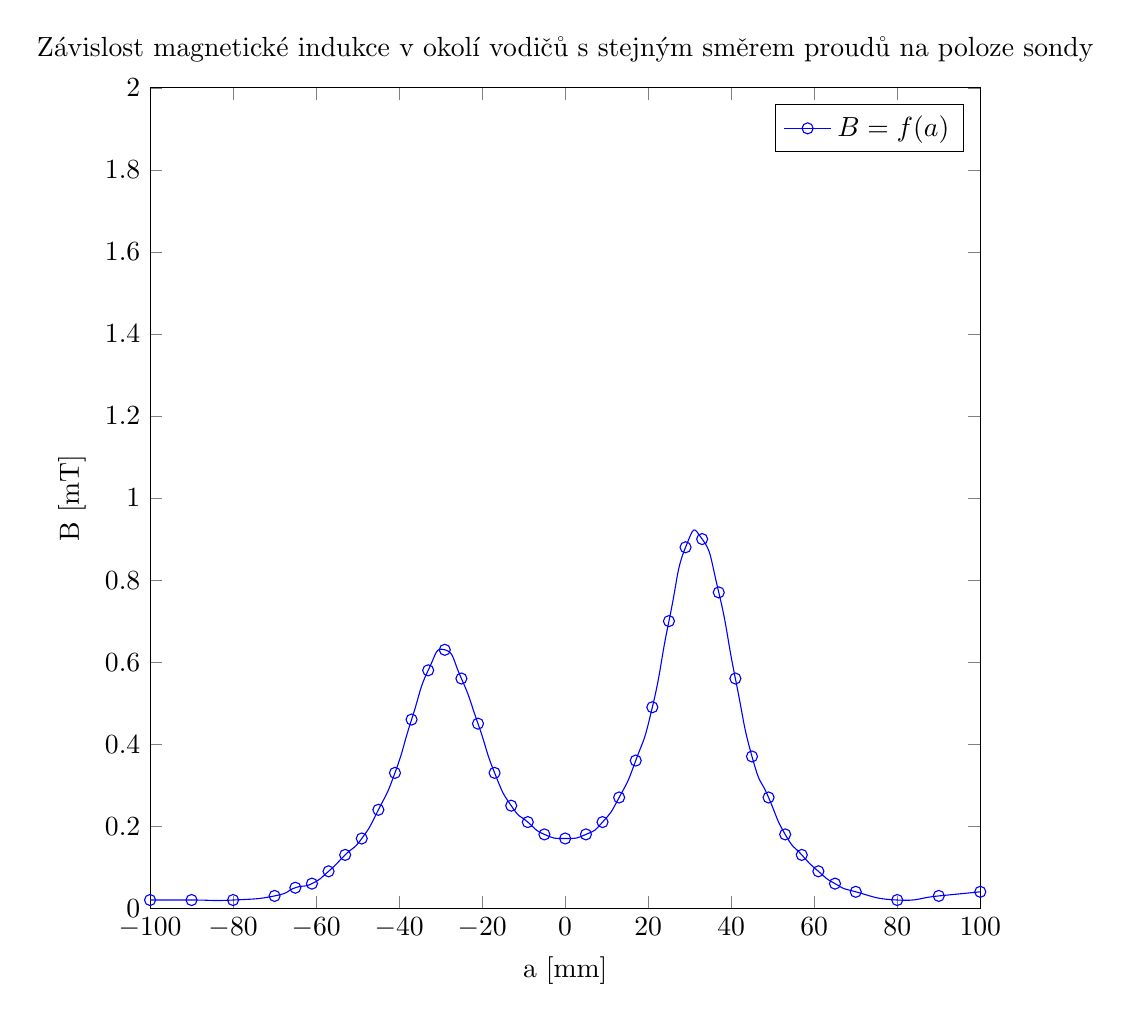
\begin{tikzpicture}[]

\begin{axis}[
    title={Závislost magnetické indukce v okolí vodičů s stejným směrem proudů na poloze sondy},
    width=\textwidth,
    height= 12cm,
    xlabel={a [mm]},
    ylabel={B [mT]},
    xmin=-100, xmax=100,
    ymin=0, ymax=2,
    xtick={-100, -80, -60, -40, -20, 0, 20 ,40, 60, 80, 100},
]

\addplot[
    color=blue,
    mark=o,
    smooth, tension=01,
    ]
    coordinates {
    (-100,0.02)
    (-90, 0.02)
    (-80, 0.02)
    (-70, 0.03)
    (-65, 0.05)
    (-61, 0.06)
    (-57, 0.09)
    (-53, 0.13)
    (-49, 0.17)
    (-45, 0.24)
    (-41, 0.33)
    (-37, 0.46)
    (-33, 0.58)
    (-29, 0.63)
    (-25, 0.56)
    (-21, 0.45)
    (-17, 0.33)
    (-13, 0.25)
    (-9,  0.21)
    (-5,  0.18)
    (0,  0.17)
    (5,  0.18)
    (9,  0.21)
    (13, 0.27)
    (17, 0.36)
    (21, 0.49)
    (25, 0.70)
    (29, 0.88)
    (33, 0.90)
    (37, 0.77)
    (41, 0.56)
    (45, 0.37)
    (49, 0.27)
    (53, 0.18)
    (57, 0.13)
    (61, 0.09)
    (65, 0.06)
    (70, 0.04)
    (80, 0.02)
    (90, 0.03)
    (100,0.04)
    };
    \addlegendentry{$B=f(a)$}

\end{axis}
\end{tikzpicture}
\end{figure}

\subsubsection{Odvození vztahu pro teoretickou hodnotu magnetické indukce souhlasného směru proudů }

\paragraph{}
Pro hodnotu magnetické indukce budeme uvažovat stejnou vzdálenost osy pohybu hallovy sodny od průsečnice středů vodičů $a_v = 0.01238m$. Oběmi rameny avšak teče rozdílný proud, protože se jejich délka liší o dvojnásobek mezery mezi středy (resp. 132mm). Vztah pro odpor tohoto vodiče je následující:
\begin{equation}
\label{eqn:r}
R = \rho \cdot \frac{l}{S}
\end{equation}
Pokud toto dosadíme do Ohmova zákonu pro proud dostaneme následující vztah:

\[ I = \frac{U\cdot S}{\rho \cdot l}\]

Jelikož je napětí, průřez i měrný odpor materiálu konstantní, můžeme je nahradit znakem $\kappa$. Porovnáme-li tedy proudy vodičů, jejichž délka se liší o 124mm, dostaneme následující poměr proudů (vodič č. 2 je o 124mm kratší). Tento poměr označíme znakem~$\theta$

\[ I_1 = \kappa \cdot l \quad I_2 = \kappa \cdot (l-0.124)\]
\[ \theta = \frac{I_1}{I_2} = \frac{\kappa \cdot l}{\kappa \cdot (l-0.124)} =  \frac{l}{l-0.124r}\]

Po dosazení do kirchoffova zákonu o proudu a do upraveného vztahu (\ref{eqn:long_wire_biot_savrat}), vynásobeným kosinem uhlu mezi $a_v$ a $a_r$ (cos$\alpha$), dostaneme následující soustavu rovnic:

\[ I_2 + \theta I_2 = 100 \]
\[ 2.10^{-7} \cdot I_2 \left(\frac{\theta}{0.01238}-\frac{1}{0.06283}\right) = 0.00063\]

Po dosazení za $I_2$:

\[ \frac{0.00063\cdot 10^{7}}{2\cdot \left(\frac{\theta \cdot 1}{0.01238}-\frac{0.1959}{0.06283}\right)} + \theta \cdot \frac{0.00063\cdot 10^{7}}{2\cdot \left(\frac{\theta\cdot 1}{0.01238}-\frac{0.1959}{0.06283}\right)} = 100 \]

Numerickým řešením této rovnice dostaneme hodnotu konstanty, a i hodnotu proudu $I_2$ a $I_1$ respektive.

\[ \theta = 0.7026 \]
\[ I_1 = 41.26 A \quad \quad I_2 = 58.74 A \]

Pro tuto problematiku lze poté odvodin následující vztah pro doplnění teoretických hodnot v tabulce:

\begin{equation}
\label{eqn:calc_oppositewire_magnetic}
B_a = 2 \cdot 10^{-7} \cdot \left(\frac{41.26\cdot \frac{a_v}{\sqrt{a_v^2+(a+0.027)^2}}}{\sqrt{0.01238^2 + (a+0.029)^2}} - \frac{58.74\cdot \frac{a_v}{\sqrt{a_v^2+(a-0.033)^2}}}{\sqrt{0.01238^2 + (a-0.033	)^2}}\right)
\end{equation}

Tento vztah není úplně přesný, jelikož zde počítáme s magnetickou indukcí v jednom bodě, ve kterém neřešíme polaritu jako u Hallovy sondy.
% Please add the following required packages to your document preamble:
% \usepackage{graphicx}
\begin{table}[H]
\centering
\resizebox{0.75\columnwidth}{!}{%
\begin{tabular}{|c|c|l|c|c|c|l|c|c|c|l|}
\hline
\textbf{a} &
  \textbf{B} &
  \multicolumn{1}{c|}{\textbf{B}} &
   &
  \textbf{a} &
  \textbf{B} &
  \multicolumn{1}{c|}{\textbf{B}} &
   &
  \textbf{a} &
  \textbf{B} &
  \multicolumn{1}{c|}{\textbf{B}} \\ \hline
\textit{{[}mm{]}} &
  \textit{{[}mT{]}} &
  \multicolumn{1}{c|}{\textit{{[}mT{]}}} &
  \textit{} &
  \textit{{[}mm{]}} &
  \textit{{[}mT{]}} &
  \multicolumn{1}{c|}{\textit{{[}mT{]}}} &
  \textit{} &
  \textit{{[}mm{]}} &
  \textit{{[}mT{]}} &
  \multicolumn{1}{c|}{\textit{{[}mT{]}}} \\ \hline
-100 & 0.02 & 0.01 &  & -25 & 0.56 & 0.56 &  & 33  & 0.90 & 0.92                  \\ \hline
-90  & 0.02 & 0.02 &  & -21 & 0.45 & 0.42 &  & 37  & 0.77 & 0.84                  \\ \hline
-80  & 0.02 & 0.03 &  & -17 & 0.33 & 0.29 &  & 41  & 0.56 & 0.65                  \\ \hline
-70  & 0.03 & 0.04 &  & -13 & 0.25 & 0.19 &  & 45  & 0.33 & 0.47                  \\ \hline
-65  & 0.05 & 0.06 &  & -9  & 0.21 & 0.11 &  & 49  & 0.27 & 0.34                  \\ \hline
-61  & 0.06 & 0.07 &  & -5  & 0.18 & 0.05 &  & 51  & 0.18 & 0.25                  \\ \hline
-57  & 0.09 & 0.09 &  & -0  & 0.17 & 0.01 &  & 57  & 0.13 & 0.19                  \\ \hline
-53  & 0.13 & 0.12 &  & 5   & 0.18 & 0.08 &  & 61  & 0.09 & 0.14                  \\ \hline
-49  & 0.17 & 0.16 &  & 9   & 0.21 & 0.14 &  & 65  & 0.06 & 0.11                  \\ \hline
-45  & 0.24 & 0.23 &  & 13  & 0.27 & 0.21 &  & 70  & 0.04 & 0.09                  \\ \hline
-41  & 0.33 & 0.32 &  & 17  & 0.36 & 0.31 &  & 80  & 0.02 & 0.05                  \\ \hline
-37  & 0.46 & 0.44 &  & 21  & 0.49 & 0.45 &  & 90  & 0.03 & 0.04                  \\ \hline
-33  & 0.58 & 0.57 &  & 25  & 0.70 & 0.64 &  & 100 & 0.04 & 0.03                  \\ \hline
-29  & 0.63 & 0.63 &  & 29  & 0.88 & 0.83 &  &     &      & \multicolumn{1}{c|}{} \\ \hline
\end{tabular}%
}
\caption{Tabulka naměřených hodnot B = f(a) při I=100A s teoretickými hodnotami}
\label{tab:namer_bfa_souhlas_teo}
\end{table}

\begin{figure}[H]
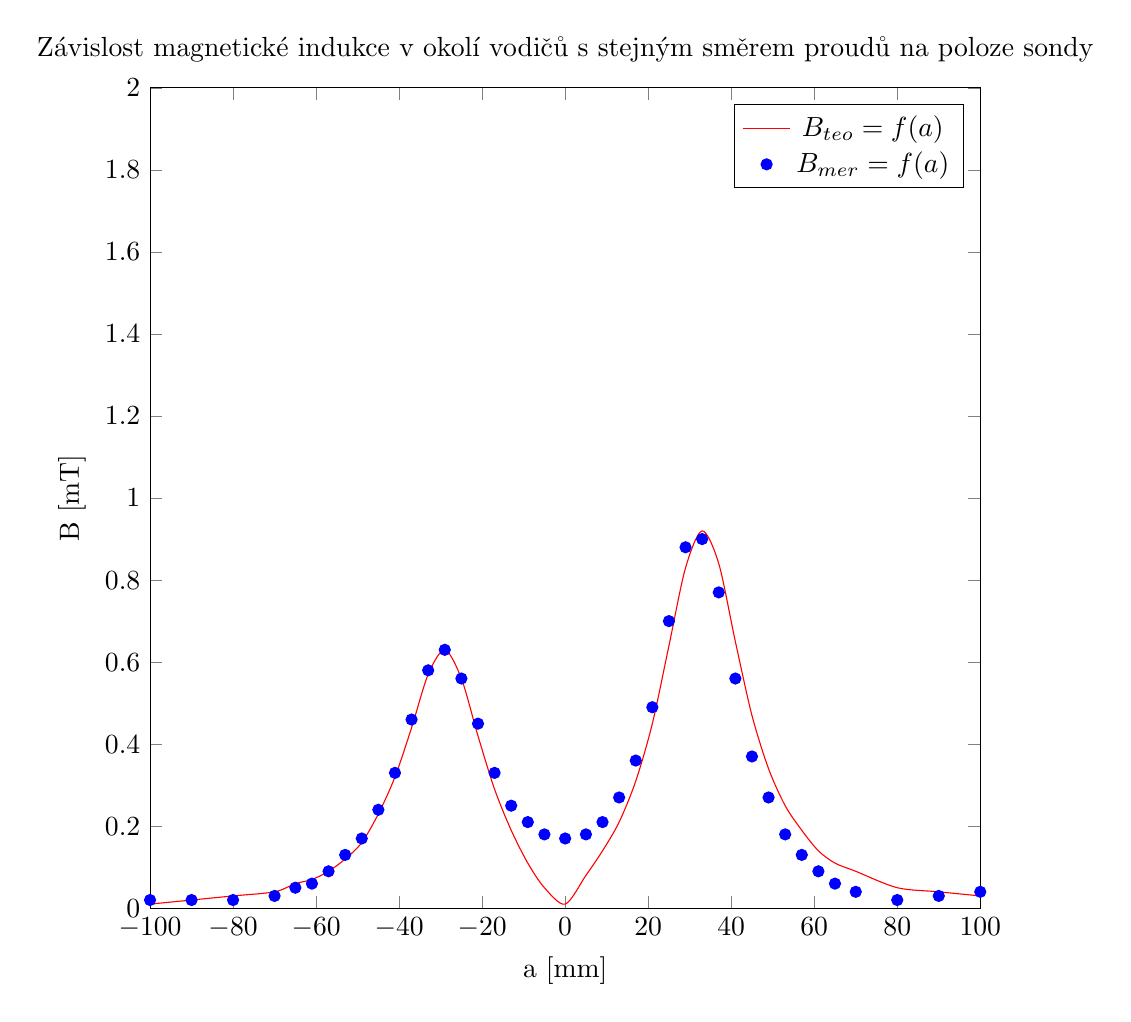
\begin{tikzpicture}[]

\begin{axis}[
    title={Závislost magnetické indukce v okolí vodičů s stejným směrem proudů na poloze sondy},
    width=\textwidth,
    height= 12cm,
    xlabel={a [mm]},
    ylabel={B [mT]},
    xmin=-100, xmax=100,
    ymin=0, ymax=2,
    xtick={-100, -80, -60, -40, -20, 0, 20 ,40, 60, 80, 100},
]
\addplot[
    color=red,
    smooth
    ]
    coordinates {
    (-100,0.01)
    (-90, 0.02)
    (-80, 0.03)
    (-70, 0.04)
    (-65, 0.06)
    (-61, 0.07)
    (-57, 0.09)
    (-53, 0.12)
    (-49, 0.16)
    (-45, 0.23)
    (-41, 0.32)
    (-37, 0.44)
    (-33, 0.57)
    (-29, 0.63)
    (-25, 0.56)
    (-21, 0.42)
    (-17, 0.29)
    (-13, 0.19)
    (-9,  0.11)
    (-5,  0.05)
    (0,  0.01)
    (5,  0.08)
    (9,  0.14)
    (13, 0.21)
    (17, 0.31)
    (21, 0.45)
    (25, 0.64)
    (29, 0.83)
    (33, 0.92)
    (37, 0.84)
    (41, 0.65)
    (45, 0.47)
    (49, 0.34)
    (53, 0.25)
    (57, 0.19)
    (61, 0.14)
    (65, 0.11)
    (70, 0.09)
    (80, 0.05)
    (90, 0.04)
    (100,0.03)
    };
\addplot[
    color=blue,
    only marks
    ]
    coordinates {
    (-100,0.02)
    (-90, 0.02)
    (-80, 0.02)
    (-70, 0.03)
    (-65, 0.05)
    (-61, 0.06)
    (-57, 0.09)
    (-53, 0.13)
    (-49, 0.17)
    (-45, 0.24)
    (-41, 0.33)
    (-37, 0.46)
    (-33, 0.58)
    (-29, 0.63)
    (-25, 0.56)
    (-21, 0.45)
    (-17, 0.33)
    (-13, 0.25)
    (-9,  0.21)
    (-5,  0.18)
    (0,  0.17)
    (5,  0.18)
    (9,  0.21)
    (13, 0.27)
    (17, 0.36)
    (21, 0.49)
    (25, 0.70)
    (29, 0.88)
    (33, 0.90)
    (37, 0.77)
    (41, 0.56)
    (45, 0.37)
    (49, 0.27)
    (53, 0.18)
    (57, 0.13)
    (61, 0.09)
    (65, 0.06)
    (70, 0.04)
    (80, 0.02)
    (90, 0.03)
    (100,0.04)
    };
        \addlegendentry{$B_{teo}=f(a)$}

    \addlegendentry{$B_{mer}=f(a)$}

\end{axis}
\end{tikzpicture}
\end{figure}

\section{Použité přístroje}
% Please add the following required packages to your document preamble:
% \usepackage{graphicx}
\begin{table}[H]
\centering
\resizebox{0.75\columnwidth}{!}{%
\begin{tabular}{|l|l|l|l|l|}
\hline
\textbf{Název}               & \textbf{Výrobce} & \textbf{Typ} & \textbf{Rozsha}   & \textbf{Výrobní číslo} \\ \hline
Teslametr                    & PHYWE            &              & \textit{20mT}     & HIM807545              \\ \hline
Stelltrafo                   & PHYWE            &              & \textit{}         & 314649                 \\ \hline
Digitální klešťový multimetr & UNI-T            & UT201        & \textit{200/400A} & 818018781              \\ \hline
\end{tabular}%
}
\caption{Použité měřící přístroje}
\label{tab:my-tablosos}
\end{table}

\section{Závěr}
\paragraph{}
V tomto měření jsme ověřovali platnost Biotova-Savaratova zákona. To jsme prováděli pomocí hallovy sondy, kterou jsme posunovali po ose s měřítkem. V první části jsme sondu dali co nejblíže k jednotnému vodiči, a proměřovali jsme závislost magnetické indukce na proudu vodičem. Poté jsem si výpočty určil pravděpodobnou vzdálenost sondy od vodiče, a na základě tohoto jsem proložil křivkou s tímto parametrem vzdálenosti. Výsledná přímka odpovídá naměřeným hodnotám s minimální odchylkou, tudíž se tím potvrzuje teorie. \\

\indent Při druhém a třetím měření jsme prováděli měření závislosti magnetické indukce v okolí dvou paralelních vodičů. při měření č. 2 byly proudy ve vodičích opačné polarity (realizováno pomocí vodiče ve tvaru obdelníku, který byl přerušen připojením ke zdroji), a u měření č. 3 byly proudy stejné polarity, ale z důvodu odlišné délky paralelních větví jimi tekl rozdílný proud. Tato problematika je popsána ve zpracování hodnot. Z grafů teoretických a naměřených hodnot lze pozorovat, že se hodnoty mezi vodiči neshodují s teorií. To je pravděpodobně způsobeno špatným provedením hallovy sondy, která měří pouze v jednom směru. Pokud si toto uvědomíme, průběhy budou dávat smysl. Tudíž můžeme uvažovat teorii opět za pravdivou, a můžeme považovat Biot-Savaratův zákon za platný.


\end{document}

